\documentclass{beamer}
%% Possible paper sizes: a0, a0b, a1, a2, a3, a4.
%% Possible orientations: portrait, landscape
%% Font sizes can be changed using the scale option.
\usepackage[portrait,size=a3,scale=1.4]{beamerposter}
\usetheme{LLT-poster}
 \usecolortheme{ComingClean}
%\usecolortheme{Entrepreneur}
% \usecolortheme{ConspiciousCreep}  %% VERY garish.
\usepackage{gensymb}
\usepackage[utf8]{inputenc}
\usepackage[T1]{fontenc}
\usepackage{libertine}
\usepackage[scaled=0.92]{inconsolata}
\usepackage[libertine]{newtxmath}

\usepackage{mwe}
\setbeamertemplate{caption}[numbered]
\author[p.duernay@protonmail.com]{Philipp Duernay}
\title{Robust and Lightweight Gate Detection for Autonomous MAV Race}
\institute{TU Delft}
% Optional foot image
\footimage{		
\includegraphics[height=2cm]{fig/tudelft}  
\includegraphics[height=2cm]{fig/mavlab} 
	
\includegraphics[height=2cm]{fig/prgroup}}

\begin{document}
\begin{frame}[fragile]
\begin{columns}[T]

%%%% First Column
\begin{column}{.33\textwidth}

	
\begin{block}{Overview}
 Micro-Air-Vehices (MAV) racing poses severe challenges to vision algorithms. The amount of computational resources are limited and the processing needs to be done fast by definition. In the most advanced MAV race at the yearly IROS conference the race court consists of several gates that need to be passed one after another (Figure 3). These gates can be used as reference point to determine the MAVs position. This thesis investigates the development of a learning based gate detector. The preliminary research questions are summarized in \textbf{Research Questions}.

\end{block}

%----------------------------------------------------------------------------------------
\begin{block}{Approach}
	\label{box::method}
	We use a state of the art object detector \cite{Redmon} and exploit the fact that we only need to detect one object that consists of quite simple shapes to simplify the architecture. E.g. we reduce the width and depth of the model (GateNet10) and use larger pooling regions in the higher order layers (GateNet12).
	
	We generate training images in simulation to train the model (Figure 2). By generating a variety of backgrounds with different lightning conditions and backgrounds our method can learn a robust representation. By simulating the effects of a real MAV camera e.g. distortion and motion blur we reduce the reality gap. 
\end{block}

\begin{block}{Intermediate Results}
	
	Figure 1 shows precision over recall as an average over 1000 images. We see how our method can perform equally well with only 0.06-1.4 \% of the parameters. However, the best performing model is still the deepest one. 
	
	Table 1 shows the mean precision across all recall levels (mAP) and the inference time of the network as an average of 1000 images. Experiments have been taken out on a nVidia Pascal with 12 GB RAM. We see how the model simplification increases speed by factor 2.5 - 3.2. This is way lower than the reduction in weights and not enough to run the network on an MAV yet.

	\centering
	\begin{table}[width=\textwidth]
		\caption{Results}
		\label{tab:models}
		\begin{tabular}{|p{3cm}|p{1cm}|p{1cm}|p{2cm}|p{2cm}|}
			\hline
			Name 		&  mAP   & T{[}ms{]} & weights &   layers   \\ \hline
			GateNet10   &  0.874 & 7.02      & 723417      &   9 \\ \hline
			GateNet12   &  0.863 & 5.43      & 285385       &   8\\ \hline
			TinyYolo    &  0.869 & 8.2       & 15867885      &   9\\ \hline
			Yolo        &  0.881 & 17.45     & 50676436       &   23\\ \hline
		\end{tabular}
	\end{table}

\end{block}
\begin{alertblock}{References}
	
	\nocite{*} % Insert publications even if they are not cited in the poster
	\small{\bibliographystyle{unsrt}
		\bibliography{sample}\vspace{0.75in}}
	
\end{alertblock}

\end{column}



%%%% This is the THIRD column
\begin{column}{.66\textwidth}

	
	\begin{block}{Research Questions}
		
		\begin{enumerate}
			\item \textbf{How can we robustly detect objects that consist mainly of lines and edges and are largely covered by background, namely the gates in a MAV race?}
			\item \textbf{How can we deal with the limited amount of available training data?}
			\item \textbf{How can we deal with the limited computational resources on the MAV?}
		\end{enumerate}
		
		
	\end{block}
\begin{figure}

	\centering
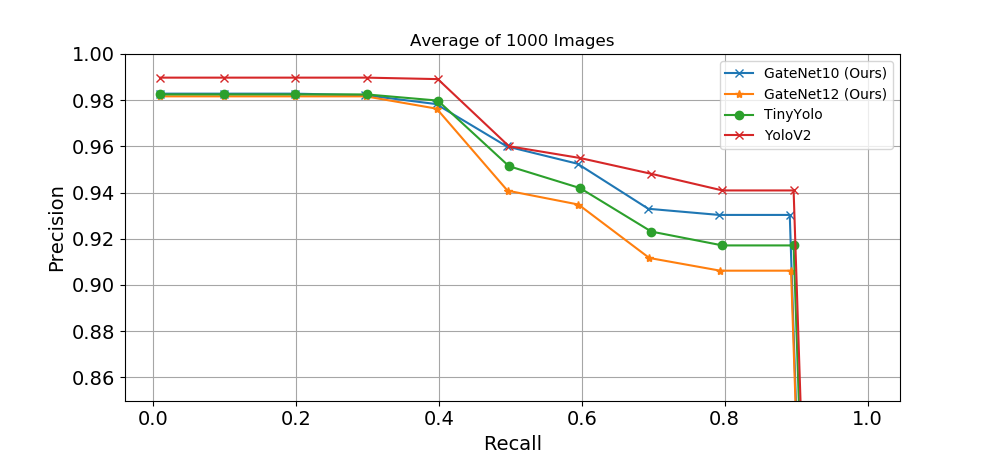
\includegraphics[width=\textwidth]{fig/pr}
\caption{Methods Compared}
\label{fig:pr}

		\begin{minipage}{0.4\textwidth}
		\centering
		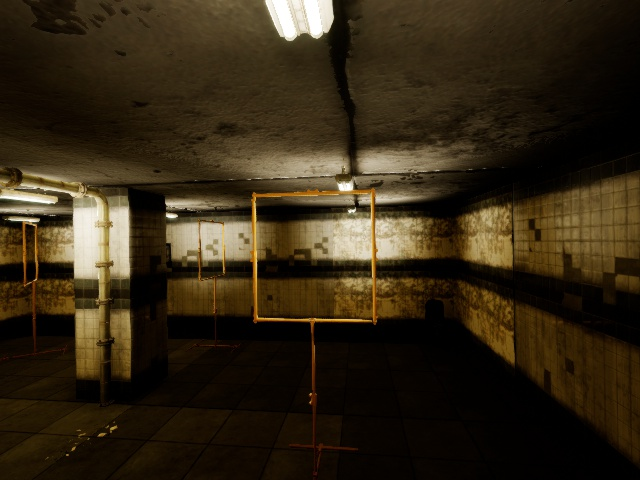
\includegraphics[height=6.5cm]{fig/sim}
		\caption{Example of simulated image}
		\label{fig:sim}
	\end{minipage}
	\hfill
\begin{minipage}{0.5\textwidth}
	\centering
	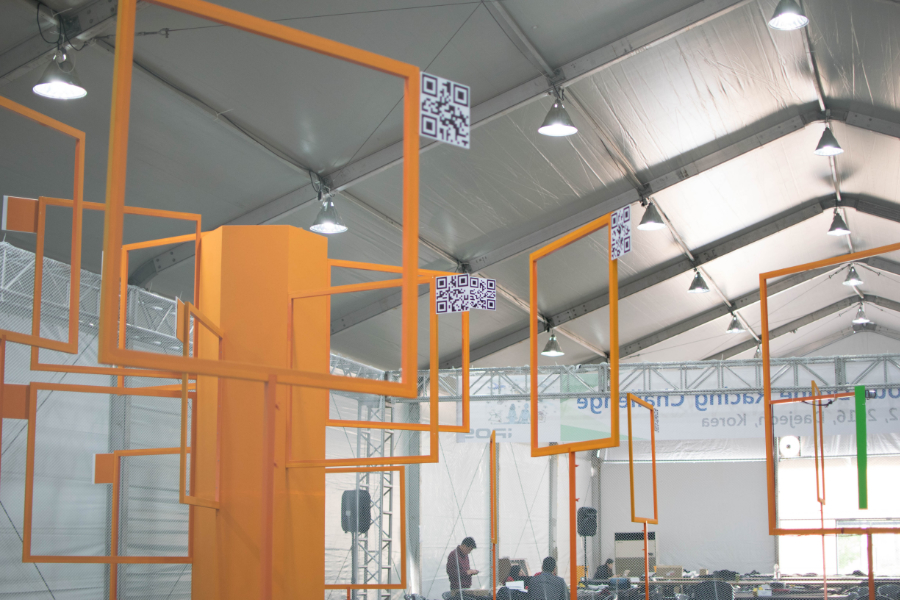
\includegraphics[height=6.5cm]{fig/iros-pic11}
	\caption{Race Court at IROS2011}
	\label{fig:iros}
\end{minipage}
	
\hfill





\end{figure}




%----------------------------------------------------------------------------------------
%   REFERENCES
%----------------------------------------------------------------------------------------






\end{column}
%%%% Second Column


\end{columns}





\end{frame}
\end{document}